\begin{appendix}

% ================================================================
\chapter{Architecture Diagrams} \label{appendix:architectures}
% ================================================================
This appendix provides the complete structural diagrams for the deep learning architectures utilized in this thesis.

\begin{figure}[H]
    \centering
    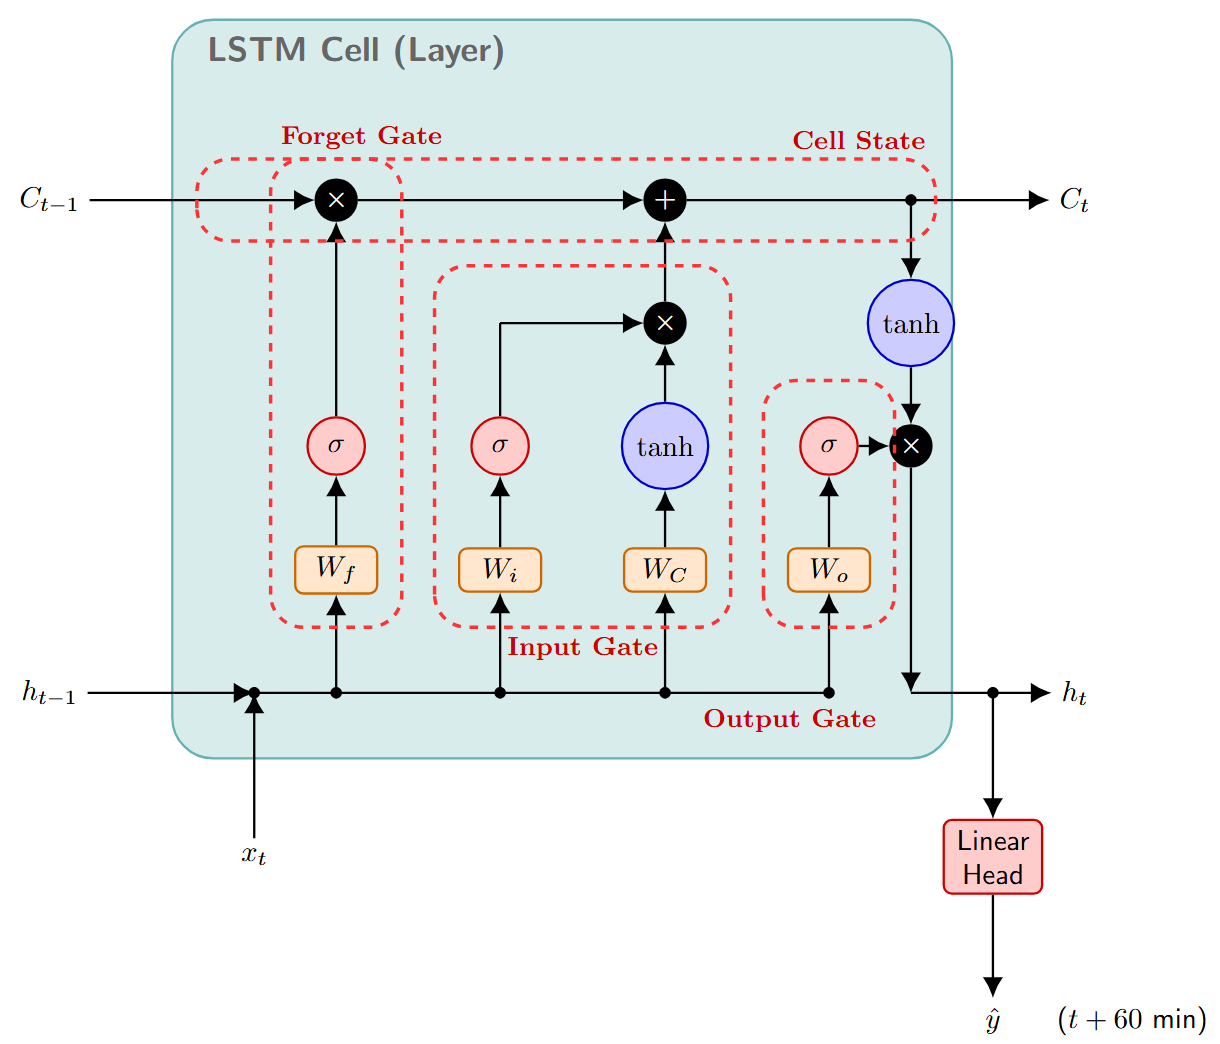
\includegraphics[width=0.9\textwidth]{lstm_cell.png}
    \caption[Architecture of the LSTM model]{Architecture of the LSTM model used as the recurrent baseline. The input is a 24-step lookback window representing 120~minutes of CGM data.}
    \label{fig:app:lstm_arch}
\end{figure}

\begin{figure}[H]
    \centering
    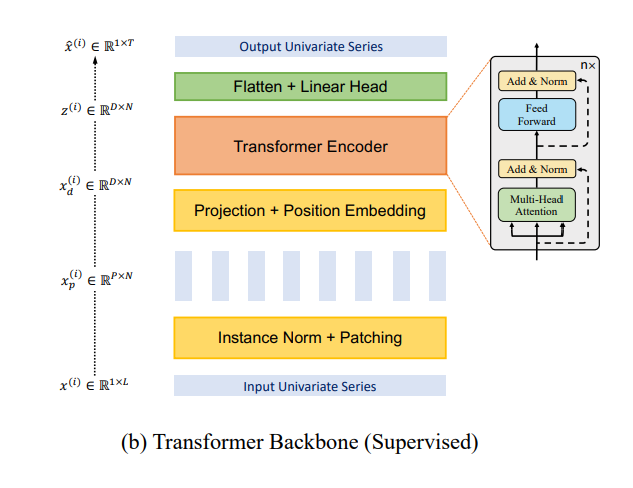
\includegraphics[width=0.9\textwidth]{patchtst_arch_b.png}
    \caption[Architecture of the PatchTST model]{Architecture of the PatchTST model adapted to the CGM setting, incorporating Reversible Instance Normalization (RevIN).}
    \label{fig:app:patchtst_arch}
\end{figure}

% ================================================================
\chapter{Detailed Evaluation Metrics} \label{appendix:detailed_metrics}
% ================================================================
This section contains supplementary figures and detailed numerical breakdowns that support the aggregated findings presented in Chapter~\ref{ch:experiments}.

\begin{figure}[htb]
    \centering
    % TODO: Replace with the actual detailed metrics figure (formerly Figure 4.5)
    \fbox{\parbox[c][45mm][c]{0.7\textwidth}{\centering\itshape
        Placeholder for \texttt{detailed\_metrics\_figure.png}.\\[3pt]
        Detailed numerical breakdown / Confusion Counts.}}
    \caption{Detailed numerical breakdown of the event detection metrics across the evaluated tolerance windows.}
    \label{fig:app:detailed_metrics}
\end{figure}

% ================================================================
\chapter{Hyperparameter Details} \label{appendix:hyperparams}
% ================================================================
\begin{planned}
    \item Specification of the final locked architecture parameters derived from the designated tuning patient.
    \item Full description of the Optuna search spaces explored for both architectures.
\end{planned}

\end{appendix}